% ----------------------------------------------------------------------
% Date: April 4th, 2016
% Author: Roberto Metere
% Project: Beamer template for Strathclyde University
%
% Copyright (C) 2016 Roberto Metere
% ----------------------------------------------------------------------
%

% examples on/off
\newif\ifexamples
%\examplestrue

% General settings
\documentclass[slidestop,compress,9pt]{beamer}
\usepackage[UKenglish]{babel}
\usepackage[UKenglish]{isodate}
\usepackage[utf8]{inputenc}
\usepackage[main]{strathclyde}
% \usepackage[tech, colour]{strathclyde}
%\usepackage[main, xcolor, strathbg]{strathclyde}
% \usepackage[eng]{strathclyde}
% \usepackage[hass]{strathclyde}
% \usepackage[bus]{strathclyde}
\usepackage{hyperref}
\definecolor{links}{HTML}{2A1B81}
\hypersetup{colorlinks=true,allcolors=links}

% Code listings and pseudocode
\usepackage{listings}
\usepackage{algpseudocode}
\usepackage{algorithm}

% Mathematical formulas
\usepackage{mathtools}
\usepackage{bm}
\setcounter{MaxMatrixCols}{20}

% Graphics and figures
\usepackage{graphicx}
\graphicspath{{figures/}}
\setbeamertemplate{caption}[numbered]
\usepackage{fancybox}
\usepackage{pgfplots}

% Tikz
\usepackage{tikz}
\usepackage{tikz-3dplot}
\usetikzlibrary{shapes.geometric, arrows}

% For redefinition of texttt
%\let\textttorig\texttt
\usepackage[scaled=1.0]{couriers}

% Numbered sections
\setbeamertemplate{section in toc}[sections numbered]
\setbeamertemplate{subsection in toc}[subsections numbered]
\setbeamertemplate{subsubsection in toc}[subsubsections numbered]

% Listings
\definecolor{cident}{rgb}{0.0,0.0,0.0}
\definecolor{ckeyw}{rgb}{0,0,0.8}
\definecolor{ccomm}{rgb}{0,0.8,0}
\definecolor{cstr}{rgb}{0.8,0,0}
\definecolor{myyellow}{rgb}{0.99,0.76, 0.0}
\definecolor{mymagenta}{rgb}{1.0, 0.0, 1.0}

\lstset{language=[LaTeX]{TeX},
  basicstyle=\normalsize\ttfamily,
  keywordstyle=\color{ckeyw}\bfseries,
  identifierstyle=\color{cident}\bfseries,
  commentstyle=\color{ccomm},
  stringstyle=\color{cstr},
  showstringspaces=false,
  breaklines=true,
  breakatwhitespace=true,
  tabsize=2,
  mathescape = false,
  columns=flexible,
  escapeinside={<@}{@>}
%   numbers=left,
%   stepnumber=1,
%   firstnumber=1,
%   numberfirstline=true,
  }

\title[Strathclyde Research Software Engineers]{\textbf{Git}}
\subtitle{An Introduction to the Version Control System }
\author[]{Oliver Henrich \\[5pt] 
\small Email: \href{mailto:oliver.henrich@strath.ac.uk}{oliver.henrich@strath.ac.uk}\\
\small Email: \href{mailto:rse-help@lists.strath.ac.uk}{rse-help@lists.strath.ac.uk}}
\institute{\textbf{\large Strathclyde Research Software Engineers}}
\date{\today}
\strathsetidentity{Strathclyde}{Research Software Engineering}

\setlength{\frametitlemargin}{1mm}

\begin{document}


%\renewcommand<>{\texttt}[1]{%
%  \only#2{\textttorig{#1}}%
%}

\renewcommand<>{\texttt}{\only#1{\beameroriginal{\texttt}}}

% ==============================================================
% --- Welcome frame
% ==============================================================
\begin{frame}[plain]
\maketitle
\end{frame}

% ==============================================================
% --- TOC
% ==============================================================

\begin{frame}[allowframebreaks,plain]
\emptyframetitle
{\Large Table of Contents}
\tableofcontents

\end{frame}

% ==============================================================
% --- Content
% ==============================================================

% ==============================================================
% --- Git
% ==============================================================
\section{Automated Version Control}\hypertarget{sec1}{}
\setcounter{framenumber}{0}

\begin{frame}[fragile]
\frametitle{Why version control?}

  \begin{columns}

    \begin{column}{0.6\textwidth}
      Problems
      \begin{itemize}
        \small
        \item Multiple, nearly identical versions of the same document
        \item Tracking changes is not an option for source code
        \item No protection against accidental deletion
      \end{itemize}
      \vspace{0.15cm}
      Version control systems 
      \begin{itemize}
        \small
        \item {\bf start} with a base version of the document
        \item {\bf record} changes you make each step of the way
        \item can {\bf revert} to any previous versions if necessary
        \item {\bf never lose} a previous state of your document
        \item allow many people to {\bf work in parallel}
      \end{itemize}
    \end{column}

    \begin{column}{0.4\textwidth}
    \begin{figure}[h]
    
\includegraphics[width=0.9\textwidth]{sec1/comic_version_control.png}
    \end{figure}
    \end{column}

  \end{columns}

\end{frame}

\begin{frame}[fragile]
\emptyframetitle
  \begin{columns}
    \begin{column}{0.33\textwidth}
{\bf Sequential changes}
      \begin{figure}[h]
      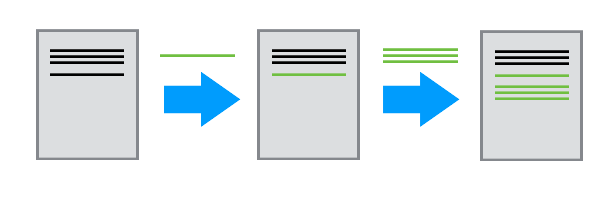
\includegraphics[width=1.0\textwidth]{sec1/change.png}
      \end{figure}
      Start at the base document, apply each change, arrive at the more recent version
    \end{column}
    \begin{column}{0.33\textwidth}
{\bf Diverging versions}
      \begin{figure}[h]
      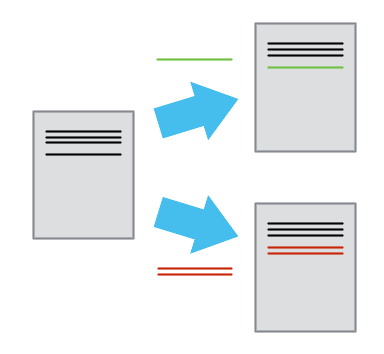
\includegraphics[width=1.0\textwidth]{sec1/versions.png}
      \end{figure}
      Two users can make independent sets of changes on the same document
    \end{column}
    \begin{column}{0.33\textwidth}
{\bf Merge versions}
      \begin{figure}[h]
      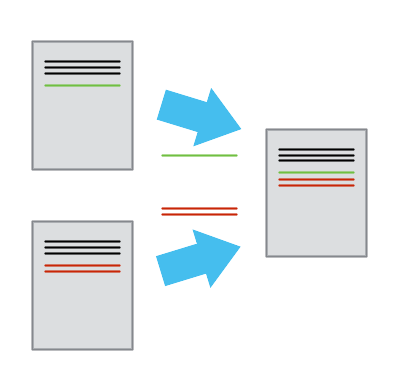
\includegraphics[width=1.0\textwidth]{sec1/merge.png}
      \end{figure}
      Incorporate two sets of changes into the same base document
    \end{column}

  \end{columns}

\end{frame}

\begin{frame}[fragile]
\emptyframetitle

\textbf{Further reasons} for using Git

\begin{itemize}
\setlength\itemsep{10pt}
  \item \textbf{Sequence of clean, logical patches}, not uncorrelated random changes
  \item Git as starting point for \textbf{automated unit and regression tests}, e.g. via Gitlab, GitHub
  \item Git for \textbf{reproducing results}, not only source code
  \begin{itemize}
    \normalsize
    \item configuration changes
    \item data sets
    \item anything in ASCII
    \item \LaTeX source code
  \end{itemize}
  \item \textbf{Collaboration} as everyone uses Git
\end{itemize}
\end{frame}

\begin{frame}[fragile]
\emptyframetitle

Example: determine buggy version via bisection\\[7pt]

\textbf{Manually}
\begin{enumerate}
  \item Define (latest) buggy version \texttt{B}
  \item Find some working version \texttt{W}
  \item Check out intermediate version \texttt{I} half-way between \texttt{B} and \texttt{W}, build, run\label{int_man}
  \begin{itemize}
    \normalsize
    \item Working? $\Rightarrow$ \texttt{W = I}
    \item Not working? $\Rightarrow$ \texttt{B = I}
  \end{itemize}
  \item Goto \ref{int_man}
  \item Identfied buggy version?
  \begin{itemize}
    \normalsize
    \item Identify change that causes the bug
    \item Do \texttt{diff} on \textbf{all} source code files
    \item \textbf{Can take hours, days or weeks} depending on code size and differences
  \end{itemize}
\end{enumerate}

\end{frame}

\begin{frame}[fragile]
\emptyframetitle

Another example: determine buggy version via bisection\\[7pt]

\textbf{Automated}
\begin{enumerate}
  \item Start bisect wizzard with \texttt{git bisect start}
  \item Define buggy version with \texttt{git bisect bad someCommitID}
  \item Define working version with \texttt{git bisect good anotherCommitID}
  \item Git checks out intermediate version, build, run\label{int_aut}
  \begin{itemize}
    \normalsize
    \item Working? $\Rightarrow$ \texttt{git bisect good}
    \item Not working? $\Rightarrow$ \texttt{git bisect bad}
  \end{itemize}
  \item Git goes to \ref{int_aut}
  \item Identfied buggy version?
  \begin{itemize}
    \normalsize
    \item \textbf{Read associated change}
    \item \textbf{Takes seconds!}
  \end{itemize}
\end{enumerate}


\end{frame}


% ==============================================================
% --- Git
% ==============================================================
\section{Basic Tasks}\hypertarget{sec2}{}

\begin{frame}[fragile]
\emptyframetitle
  In this section
  \begin{itemize}
    \item \hyperlink{sec2.1}{Setting Up Git}
    \item \hyperlink{sec2.2}{Creating A Git Repository}
    \item \hyperlink{sec2.3}{Tracking Changes}
    \item \hyperlink{sec2.4}{Exploring History}
  \end{itemize}
\end{frame}

\subsection{Setting Up Git}\hypertarget{sec2.1}{}

\begin{frame}[fragile]
\emptyframetitle

  Git comes in many different forms. We use \textbf{Git on the command line}.

  \begin{itemize}
  \item It's the only place you can run \textbf{all} Git commands.
  \item If you know the command line version, you can figure out how to run the GUI version.
  \item Everyone has the same command line tools.
  \end{itemize}

  \vspace*{0.15cm}
  On Linux 
  \begin{itemize}
    \item[] \texttt{\$ sudo dnf install git-all} (Fedora) 
    \item[] \texttt{\$ sudo apt install git-all} (Debian)
  \end{itemize}
  \vspace*{0.15cm}

  On Mac 
  \begin{itemize}
    \item[] \texttt{\$ brew install git} (Homebrew) 
    \item[] \texttt{\$ port install git} (Macports)
    \item[] part of XCode IDE
  \end{itemize}
  \vspace*{0.15cm}

  On Windows 
  \begin{itemize}
    \item[] Git for Windows: \url{https://git-scm.com/download/win} 
    \item[] GitHub Desktop: \url{https://desktop.github.com}
    \item[] Git Chocolatey: \url{https://chocolatey.org/packages/git}
  \end{itemize}

\end{frame}

\begin{frame}[fragile]
\emptyframetitle
  When we use Git for the first time, we need to configure a few things.\\[0.25cm]

  Here are a few examples of configurations we will set as we get started with Git:
  \begin{itemize}
    \item your name and email address
    \item and that we want to use these settings globally (i.e. for every project)
  \end{itemize}
  On a command line, Git commands are written as \texttt{\textbf{git verb options}}, where \texttt{\textbf{verb}} is what we actually want to do and \texttt{\textbf{options}} is additional optional information which may be needed for the verb.\\[0.25cm]

  So here is how Dracula sets up his new laptop:

  \begin{lstlisting}[language=bash]
    $ git config --global user.name "Vlad Dracula"
    $ git config --global user.email "vlad@tran.sylvan.ia"
  \end{lstlisting}

\end{frame}

\begin{frame}[fragile]
\emptyframetitle

  Quite helpful and important are the commands to look up the manual\\[0.25cm] 

  For a general overview of a range of Git commands
  \begin{lstlisting}[language=bash]
    $ git --help
  \end{lstlisting}

  For a overview of specific Git command (here command = \texttt{verb})
  \begin{lstlisting}[language=bash]
    $ git verb -h
  \end{lstlisting}

  For an in-depth manual of specific Git command
  \begin{lstlisting}[language=bash]
    $ git verb --help
  \end{lstlisting}

  \vspace*{0.5cm}
  For more information please check the \textbf{Git online documentation} at
  \url{https://git-scm.com/docs}

\end{frame}

\subsection{Creating A Git Repository}\hypertarget{sec2.2}{}


\begin{frame}[fragile]
\emptyframetitle

  Create a directory in your current working directory
  \begin{lstlisting}[language=bash]
    $ mkdir git_exercise
  \end{lstlisting}

  Change to the new directory
  \begin{lstlisting}[language=bash]
    $ cd git_exercise
  \end{lstlisting}

  Create the Git repository
  \begin{lstlisting}[language=bash]
    $ git init
  \end{lstlisting}

  \begin{block}{Note}
An invisible file \texttt{.git} is created that stores all the history and dependencies of the repository.
  \end{block}

\end{frame}

\subsection{Tracking Changes}\hypertarget{sec2.3}{}

\begin{frame}[fragile]
\emptyframetitle

  Think of Git as taking snapshots of your project in a two-step process:
  \begin{itemize}
    \item \texttt{\textbf{git add}} specifies \textbf{what} will go into a snapshot
    \item \texttt{\textbf{git commit}} \textbf{takes the actual snapshot} and records it permanently
  \end{itemize}

  \begin{figure}[h]
    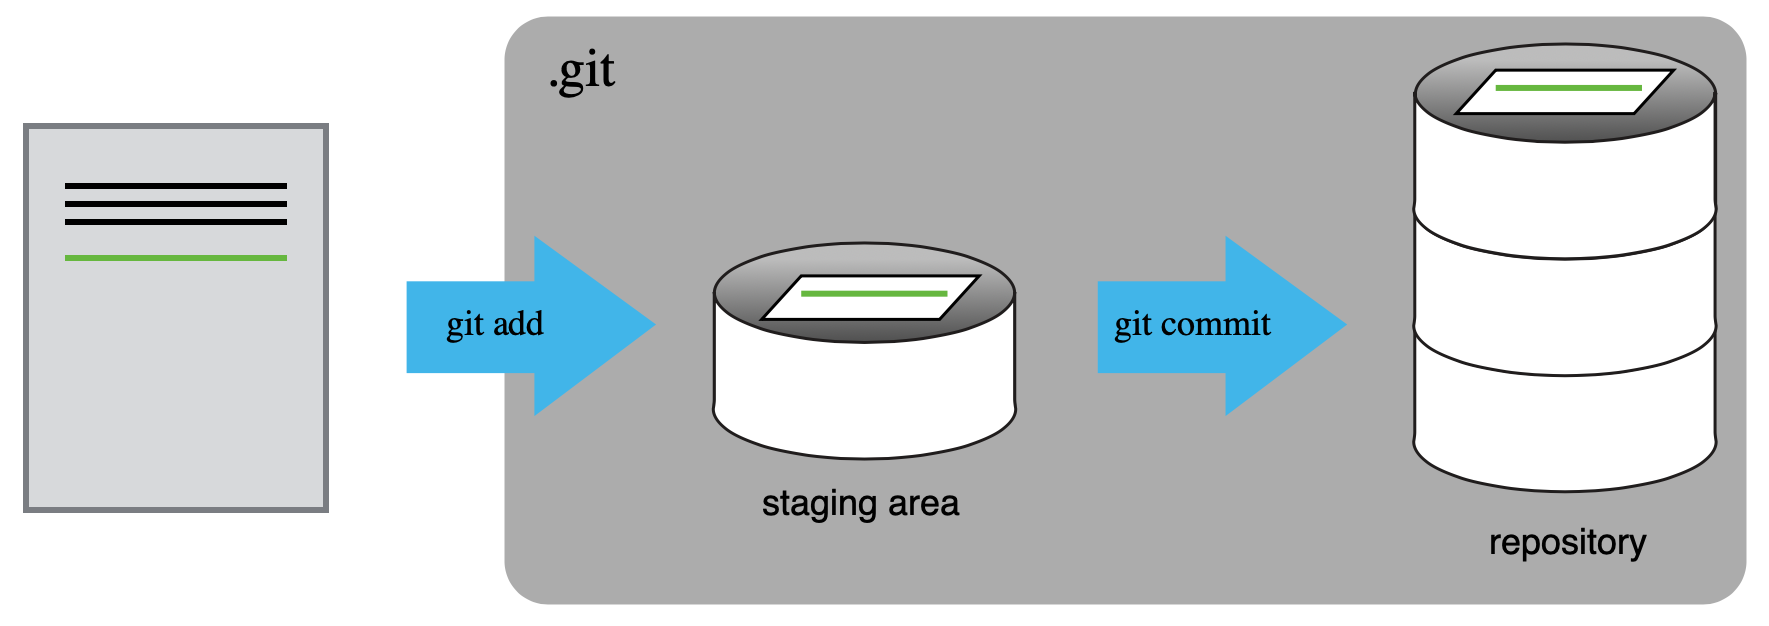
\includegraphics[width=1.0\textwidth]{sec2/git-staging-area.png}
  \end{figure}

\end{frame}

\begin{frame}[fragile]
\emptyframetitle

  It is of course possible to add multiple files (or changes thereof) before committing these, i.e. taking the snapshot.

  \begin{figure}[h]
    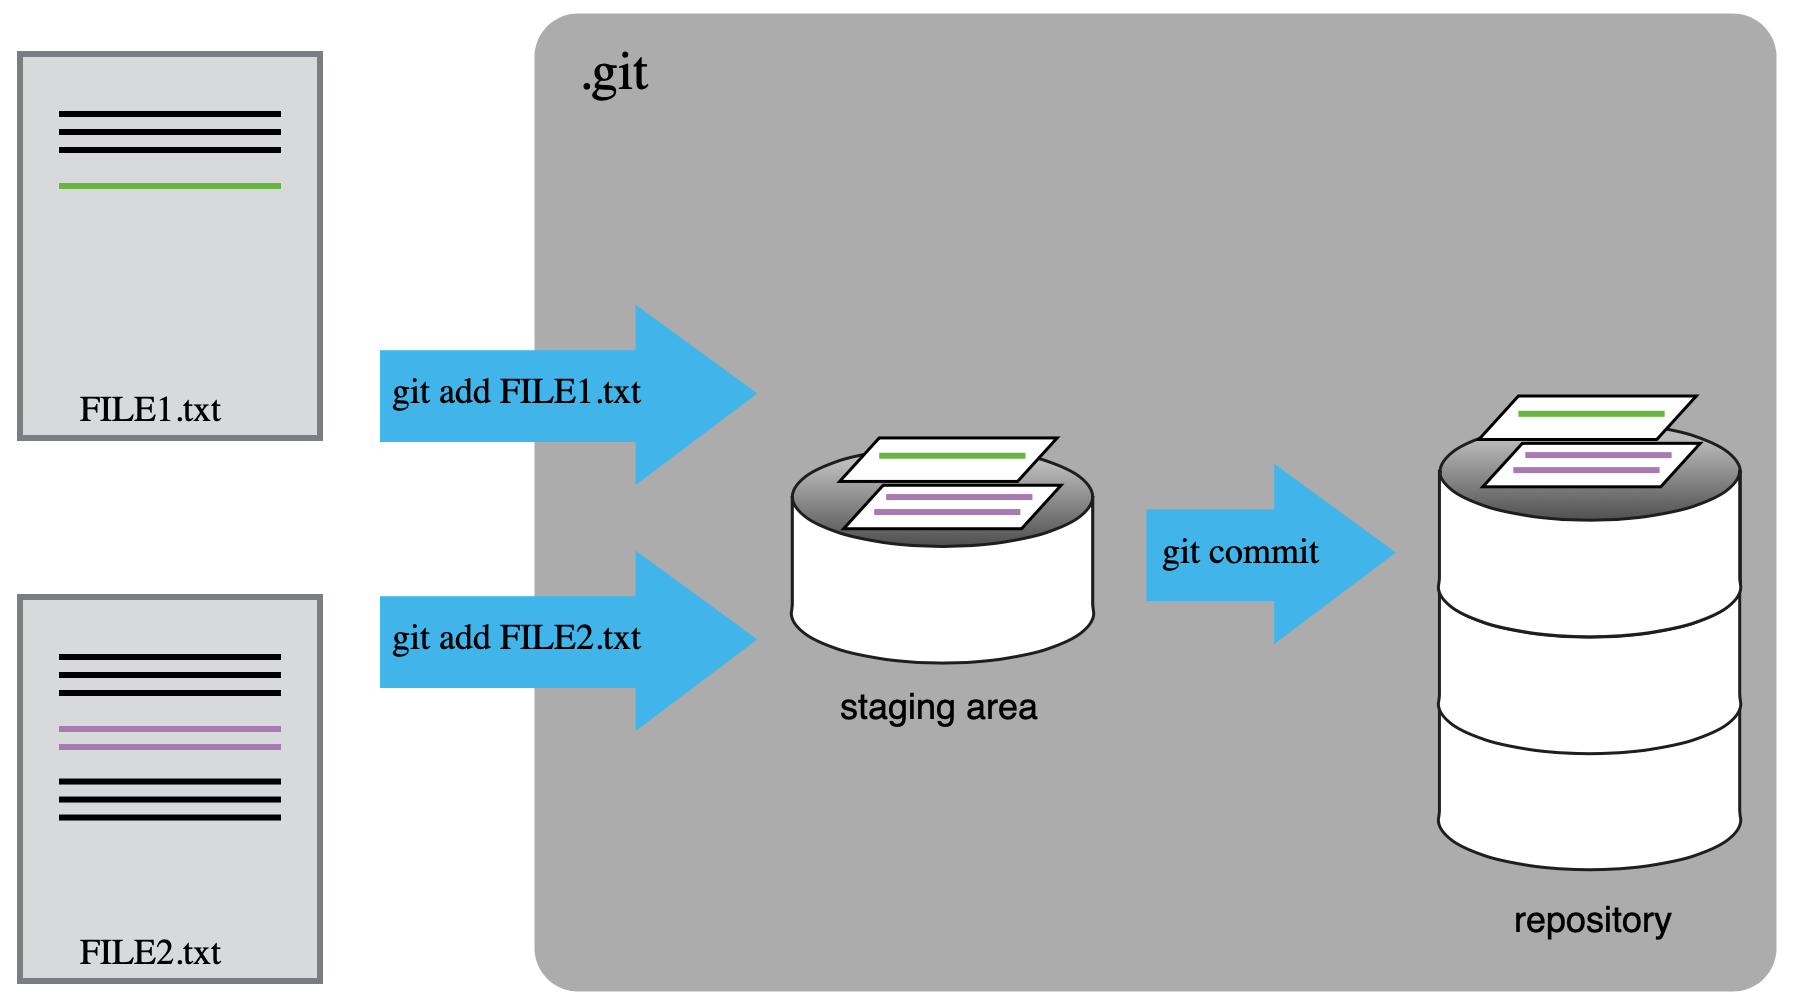
\includegraphics[width=0.95\textwidth]{sec2/git-committing.png}
  \end{figure}

\end{frame}

\begin{frame}[fragile]
\emptyframetitle

  Check the status
  \begin{lstlisting}[language=bash]
  $ git status
  \end{lstlisting}

  \begin{block}{Output if working directory / repository is brand new}
    \begin{lstlisting}[language=bash]
      On branch master
      No commits yet
      nothing to commit (create/copy files and use "git add" to track)
    \end{lstlisting}
  \end{block}

  \vspace{0.5cm}
  Now create a new file \texttt{hello\_world.py} in your working directory that prints 'Hello World!'

\end{frame}

\begin{frame}[fragile]
\emptyframetitle
  When you check the status again, you will now see there is an untracked file.
  \begin{lstlisting}[language=bash]
  $ git status
  \end{lstlisting}

  \begin{block}{Output if working directory differs, but new file is not yet being tracked}
    \begin{lstlisting}[language=bash]
      On branch master
      No commits yet
      Untracked files:
        (use "git add <file>..." to include in what will be committed)
              hello_world.py

      nothing added to commit but untracked files present (use "git add" to track)
    \end{lstlisting}
  \end{block}

\end{frame}


\begin{frame}[fragile]
\emptyframetitle
  Add your new file and start the tracking.
  \begin{lstlisting}[language=bash]
  $ git add hello_world.py
  \end{lstlisting}
  Check the status again  
  \begin{lstlisting}[language=bash]
  $ git status
  \end{lstlisting}
 
  \begin{block}{Output if working directory differs and file is being tracked}
    \begin{lstlisting}[language=bash]
      On branch master
      No commits yet
      Changes to be committed:
        (use "git rm --cached <file>..." to unstage)
              new file:   hello_world.py
    \end{lstlisting}
  \end{block}
\end{frame}

\begin{frame}[fragile]
\emptyframetitle

  Now commit the change and record it permanently.
  \begin{lstlisting}[language=bash]
  $ git commit -m 'Added new file'
  \end{lstlisting}

  \begin{block}{Output of \texttt{git commit}}
    \begin{lstlisting}[language=bash]
      [master (root-commit) b3557d4] Added new file
       1 file changed, 8 insertions(+)
       create mode 100644 hello_world.py
    \end{lstlisting}
  \end{block}
\end{frame}

\begin{frame}[fragile]
\emptyframetitle

  Check the status with \texttt{\textbf{git status}} and you get the following message:

  \begin{block}{}
    \begin{lstlisting}[language=bash]
      On branch master
      nothing to commit, working tree clean
    \end{lstlisting}
  \end{block}

  You can check the log to see your commits. The most recent appears first.

    \begin{lstlisting}[language=bash]
      $ git log
    \end{lstlisting}

  \begin{block}{}
    \begin{lstlisting}[language=bash]
      commit 249156049502e47d839735c34e31830885bc5092 (HEAD -> master)
      Author: Oliver Henrich <ohenrich@users.noreply.github.com>
      Date:   Wed Sep 2 16:56:07 2020 +0100
          Added new file
      \end{lstlisting}
  \end{block}
 
\end{frame}

\subsection{Exploring History}\hypertarget{sec2.4}{}

\begin{frame}[fragile]
\emptyframetitle

  When working with repos, you often want to \textbf{review changes before committing them} or \textbf{revert to a previous version} of the file.\\[0.25cm]

  Add an additional line to the previous \texttt{hello\_world.py} file. Check the \textbf{differences between your local and remote repository} with

  \begin{lstlisting}[language=bash]
    $ git diff
  \end{lstlisting}

  \begin{block}{Additional line \texttt{'print(`Hello Scotland!')'} in local file (+)}
    \begin{lstlisting}[language=bash]
      diff --git a/hello_world.py b/hello_world.py
      index 73fb7c3..e6f9107 100644
      --- a/hello_world.py
      +++ b/hello_world.py
      @@ -1 +1,2 @@
       print('Hello World!')
      +print('Hello Scotland!')
    \end{lstlisting}
  \end{block}

\end{frame}

\begin{frame}[fragile]
\emptyframetitle

  Commit the change 

  \begin{lstlisting}[language=bash]
    $ git add hello_world.py
    $ git commit -m 'Added additional line'
  \end{lstlisting}

  and check the differences again.

  \begin{lstlisting}[language=bash]
    $ git diff
  \end{lstlisting}

  There are no differences anymore as you committed your change.\\[0.25cm]

  Now check the status again.

  \begin{lstlisting}[language=bash]
    $ git status
  \end{lstlisting}
  \vspace*{-0.25cm}
  \begin{block}{Output of \texttt{git status}}
    \begin{lstlisting}[language=bash]
      On branch master
      nothing to commit, working tree clean
    \end{lstlisting}
  \end{block}

\end{frame}

\begin{frame}[fragile]
\emptyframetitle

  Add another line, commit the change again and check your commit log.

  \begin{columns}
    \begin{column}{0.55\textwidth}
      \begin{block}{Output of \texttt{git log}}
        \begin{lstlisting}[language=bash, basicstyle=\tiny\ttfamily]
          commit 908944eb711c90f5bd46297639b34d8fc70993f0 (HEAD -> master)
          Author: Oliver Henrich <ohenrich@users.noreply.github.com>
          Date:   Wed Sep 2 16:59:00 2020 +0100
              Added another additional line

          commit 28f46c36b5729ab26ca719cc1468b1a6e734d597
          Author: Oliver Henrich <ohenrich@users.noreply.github.com>
          Date:   Wed Sep 2 16:58:15 2020 +0100
              Added additional line

          commit 249156049502e47d839735c34e31830885bc5092
          Author: Oliver Henrich <ohenrich@users.noreply.github.com>
          Date:   Wed Sep 2 16:56:07 2020 +0100
              Added new file
        \end{lstlisting}
      \end{block}
    \end{column}

    \begin{column}{0.425\textwidth}
      \vspace*{0.cm}\\
      \textbf{All commits have a unique ID}, but Git knows a simple way to address them:\\
      \vspace*{0.4cm}
      The \textbf{last commit} appears at the top and is marked with \texttt{\textbf{HEAD}}.
      \vspace*{0.7cm}\\
      The \textbf{two previous commits} are not marked, but can be conveniently addressed with \textbf{\texttt{HEAD\textasciitilde1}} and \textbf{\texttt{HEAD\textasciitilde2}}.
    \end{column}
  \end{columns}

\end{frame}

\begin{frame}[fragile]
\emptyframetitle

  If we want to see what the differences are between the current version (\texttt{\textbf{HEAD}}) and version two commits ago, we can issue for instance

  \begin{lstlisting}[language=bash]
    $ git diff HEAD~2
  \end{lstlisting}

  \begin{block}{Additional two lines marked as different in local file (+)}
    \begin{lstlisting}[language=bash]
      diff --git a/hello_world.py b/hello_world.py
      index 73fb7c3..547a19b 100644
      --- a/hello_world.py
      +++ b/hello_world.py
      @@ -1 +1,3 @@
       print('Hello World!')
      +print('Hello Scotland!')
      +print('Hello Glasgow!')
    \end{lstlisting}
  \end{block}
\end{frame}

\begin{frame}[fragile]
\emptyframetitle

  Assume you want to obtain the previous version without the additional line.\\[0.2cm]

  First you need to \textbf{check the log for the ID of the previous commit}.

  \vspace*{-0.2cm}
  \begin{columns}
      \begin{column}{0.55\textwidth}
        \begin{block}{Output of \texttt{git log}}
          \begin{lstlisting}[language=bash, basicstyle=\tiny\ttfamily]
            commit 28f46c36b5729ab26ca719cc1468b1a6e734d597
            Author: Oliver Henrich <ohenrich@users.noreply.github.com>
            Date:   Wed Sep 2 16:58:15 2020 +0100
                Added additional line
          \end{lstlisting}
        \end{block}
      \end{column}
      \begin{column}{0.425\textwidth}
        \vspace*{0.5cm}\\
        The commit ID is the long bit starting 28f46c36b5\dots\\[0.25cm]
         It is \textbf{usually sufficient to specify only 7 digits}.
      \end{column}
    \end{columns}

  \vspace*{0.2cm}
  Use the \texttt{\textbf{git checkout}} command to retrieve a previous version.

  \begin{lstlisting}[language=bash]
    $ git checkout 28f46c36b5 hello_world.py
  \end{lstlisting}

  \textcolor{red}{\textbf{Note: Do not forget the filename at the end as this will 'detach the \texttt{HEAD}'}!}\\[0.2cm]

  To \textbf{retrieve the latest version} again use 

  \begin{lstlisting}[language=bash]
    $ git checkout master hello_world.py
  \end{lstlisting}


\end{frame}

\begin{frame}[fragile]
\emptyframetitle
  The previous command will not revert the commit (check e.g. \texttt{\textbf{git log}}).\\[0.25cm]

  To \textbf{revert an erroneous commit, first look for its ID} and use \texttt{\textbf{git revert}}.

  \begin{columns}
    \begin{column}{0.55\textwidth}
      \begin{block}{Output of \texttt{git log}}
        \begin{lstlisting}[language=bash, basicstyle=\tiny\ttfamily]
          commit 908944eb711c90f5bd46297639b34d8fc70993f0 (HEAD -> master)
          Author: Oliver Henrich <ohenrich@users.noreply.github.com>
          Date:   Wed Sep 2 16:59:00 2020 +0100
              Added another additional line

          commit 28f46c36b5729ab26ca719cc1468b1a6e734d597
          Author: Oliver Henrich <ohenrich@users.noreply.github.com>
          Date:   Wed Sep 2 16:58:15 2020 +0100
              Added additional line
        \end{lstlisting}
      \end{block}
    \end{column}

    \begin{column}{0.425\textwidth}
      \vspace*{1.cm}\\
      We want to revert the commit starting 908944eb71\dots
      \vspace*{0.8cm}\\
      We want the current version to be this one.
    \end{column}
  \end{columns}


  \begin{lstlisting}[language=bash]
    $ git revert 908944eb71 
  \end{lstlisting}

  This creates a new commit with the previous version of the file.

\end{frame}

\begin{frame}[fragile]
\emptyframetitle

\vspace*{-0.75cm}
  \begin{columns}
    \begin{column}{0.55\textwidth}
      \begin{figure}[h]
        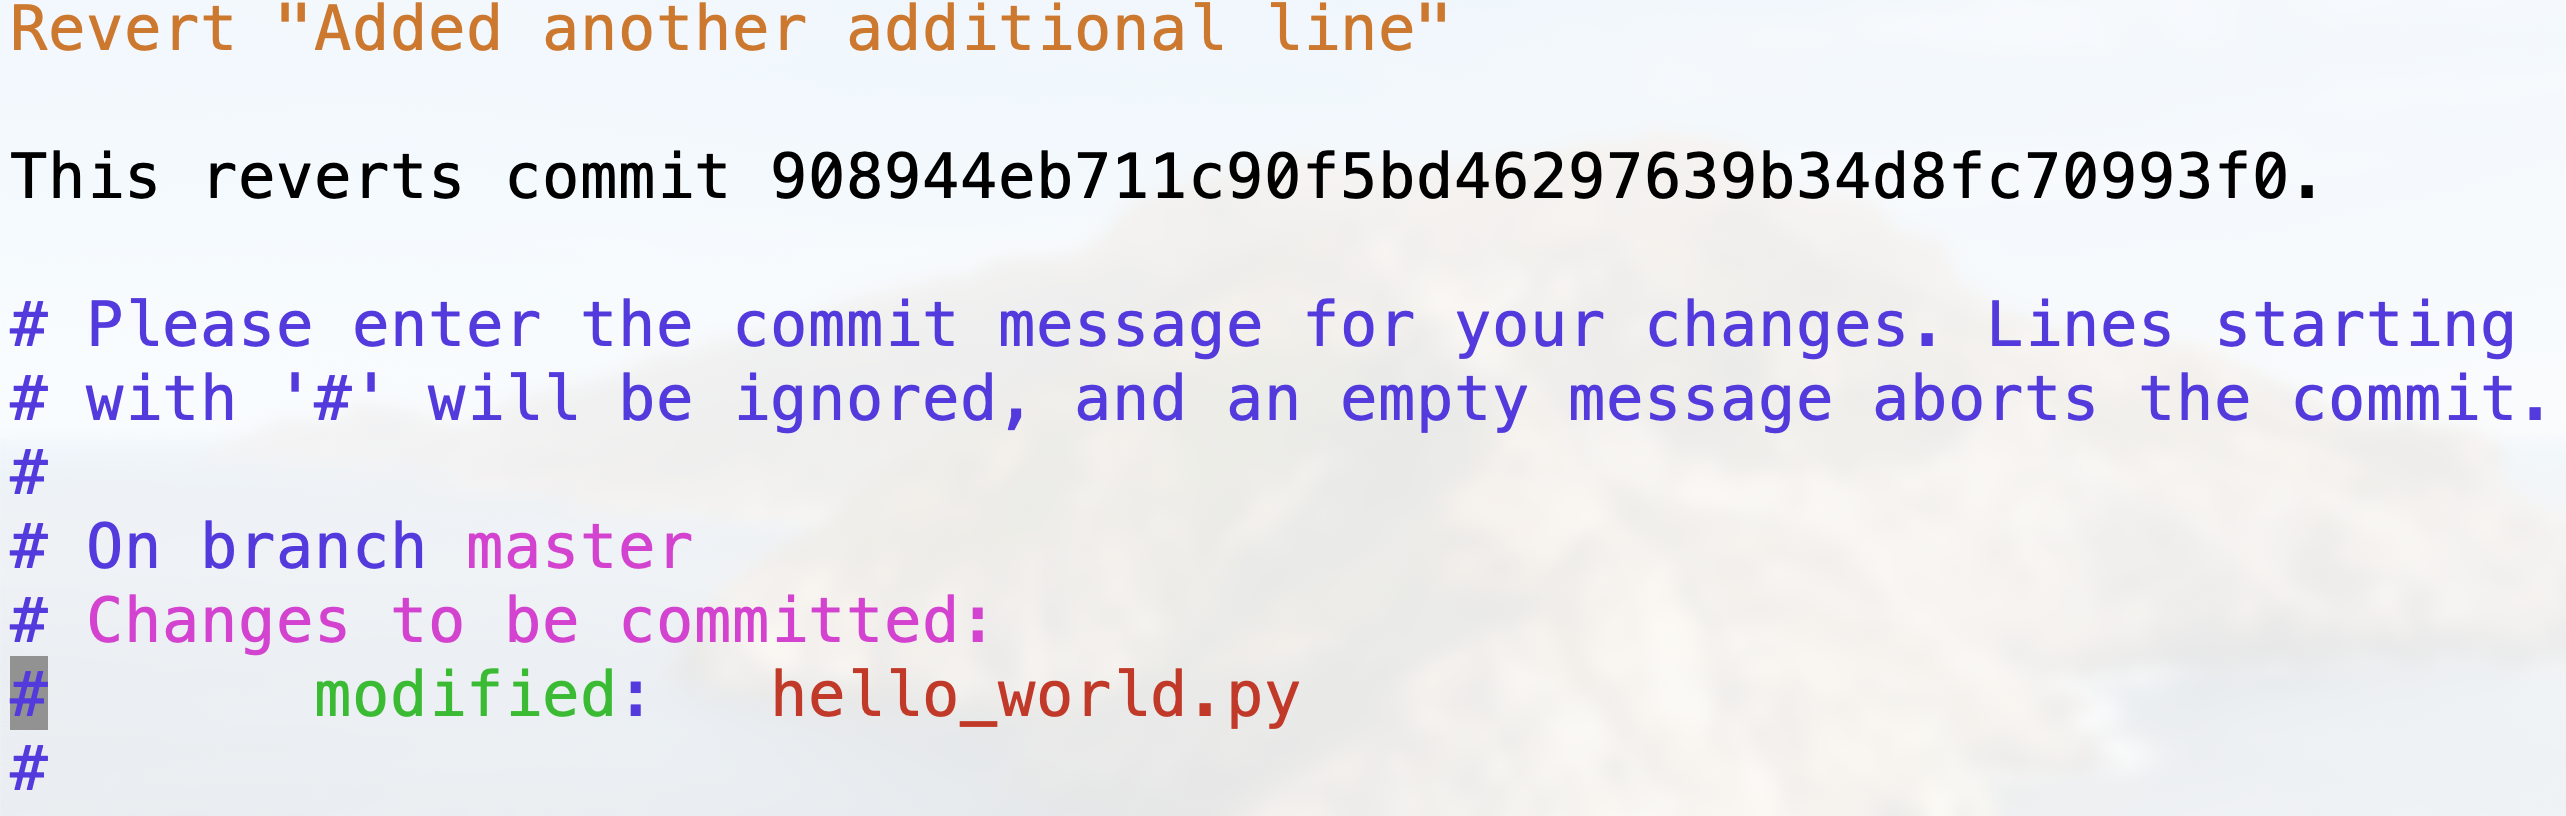
\includegraphics[width=1.0\textwidth]{sec2/git-revert.png}
      \end{figure}

    \end{column}

   \begin{column}{0.45\textwidth}
      \vspace*{0.5cm}\\
      A dialogue window opens that asks you for a message providing a template.
    \end{column}
  \end{columns}

\vspace*{-0.2cm}
  \begin{columns}
    \begin{column}{0.7\textwidth}

      \begin{block}{}
        \begin{lstlisting}[language=bash, basicstyle=\tiny\ttfamily]
          commit 15f36c3bd31f594504756326df6b3baeb2d0982c (HEAD -> master)
          Author: Oliver Henrich <ohenrich@users.noreply.github.com>
          Date:   Thu Sep 3 17:29:03 2020 +0100
              Revert "Added another additional line"
              This reverts commit 908944eb711c90f5bd46297639b34d8fc70993f0.

          commit 908944eb711c90f5bd46297639b34d8fc70993f0
          Author: Oliver Henrich <ohenrich@users.noreply.github.com>
          Date:   Wed Sep 2 16:59:00 2020 +0100
              Added another additional line

          commit 28f46c36b5729ab26ca719cc1468b1a6e734d597
          Author: Oliver Henrich <ohenrich@users.noreply.github.com>
          Date:   Wed Sep 2 16:58:15 2020 +0100
              Added additional line

          commit 249156049502e47d839735c34e31830885bc5092
          Author: Oliver Henrich <ohenrich@users.noreply.github.com>
          Date:   Wed Sep 2 16:56:07 2020 +0100
              Added new file
        \end{lstlisting}
      \end{block}
    \end{column}

     \begin{column}{0.25\textwidth}
        \vspace*{0.5cm}\\
        Your commit log has now an extra entry.
    \end{column}
  \end{columns}


\end{frame}



% ==============================================================
% --- Git
% ==============================================================
\section{Collaborative Software Development}\hypertarget{sec3}{}

\begin{frame}[fragile]
\emptyframetitle
  In this section
  \begin{itemize}
    \item \hyperlink{sec3.1}{Creating Remote Repositories on GitHub}
    \item \hyperlink{sec3.2}{Collaborating On GitHub}
    \item \hyperlink{sec3.3}{Conflicts}
  \end{itemize}
\end{frame}

\subsection{Creating Remote Repositories on GitHub}\hypertarget{sec3.1}{}

\begin{frame}[fragile]
\emptyframetitle
  One of the main reasons for using repositories is also to \textbf{collaborate with other people} and \textbf{work on the same code}. This is done through a \textbf{remote repository}. \\[0.25cm]

  \textbf{\textit{Pulling} retrieves from} the remote repo.\\
  \textbf{\textit{Pushing} deposits into} the remote repo.\\
  \textbf{\textit{Cloning} checks out a private copy} of the remote repo.
  \begin{figure}[h]
    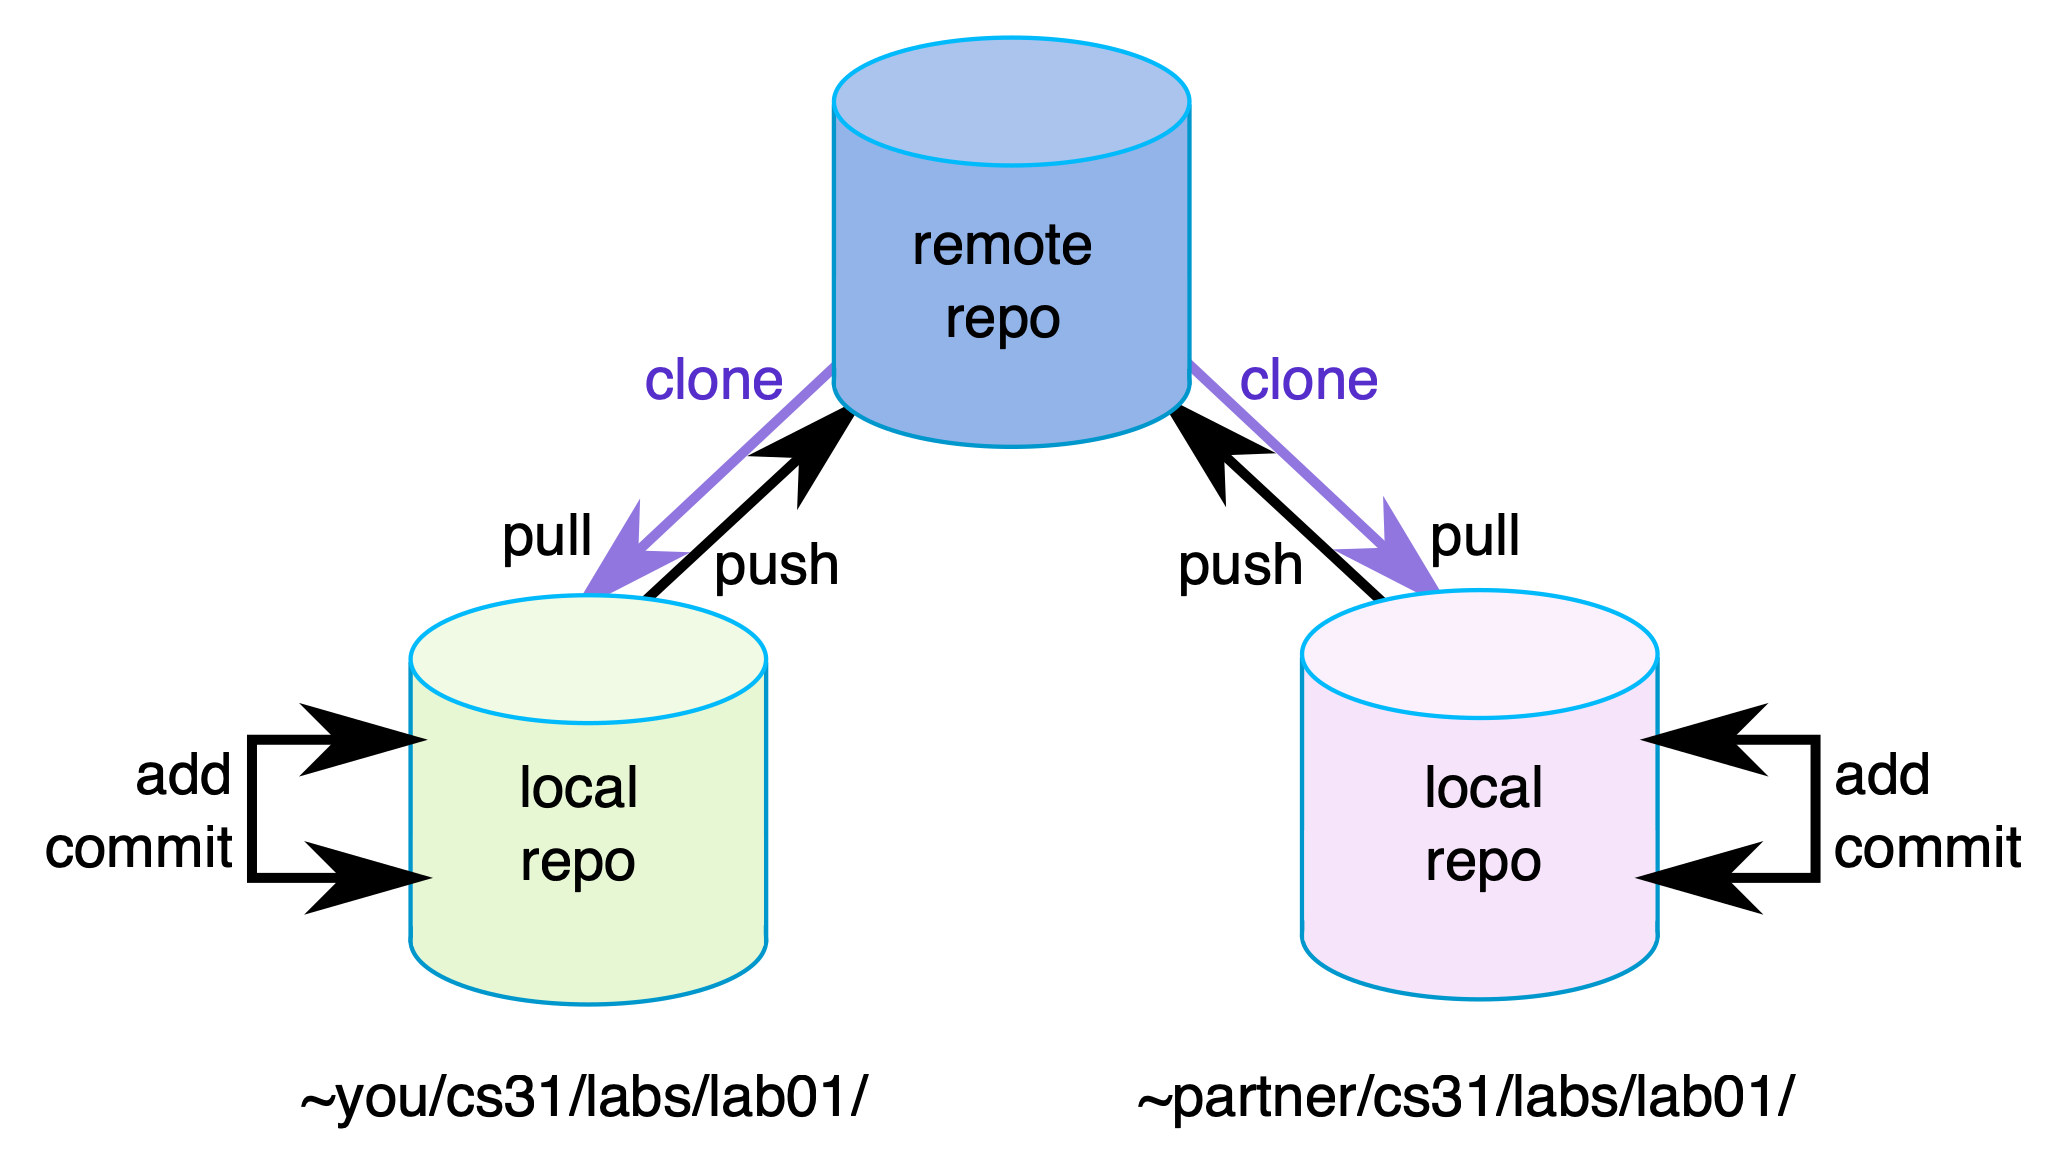
\includegraphics[width=0.7\textwidth]{sec3/git-repo_overview.png}
  \end{figure}

\end{frame}

\begin{frame}<presentation:0>[fragile]
\emptyframetitle
  We will use \textbf{GitHub} available at \textbf{\url{https://github.com}}

  \begin{figure}[h]
    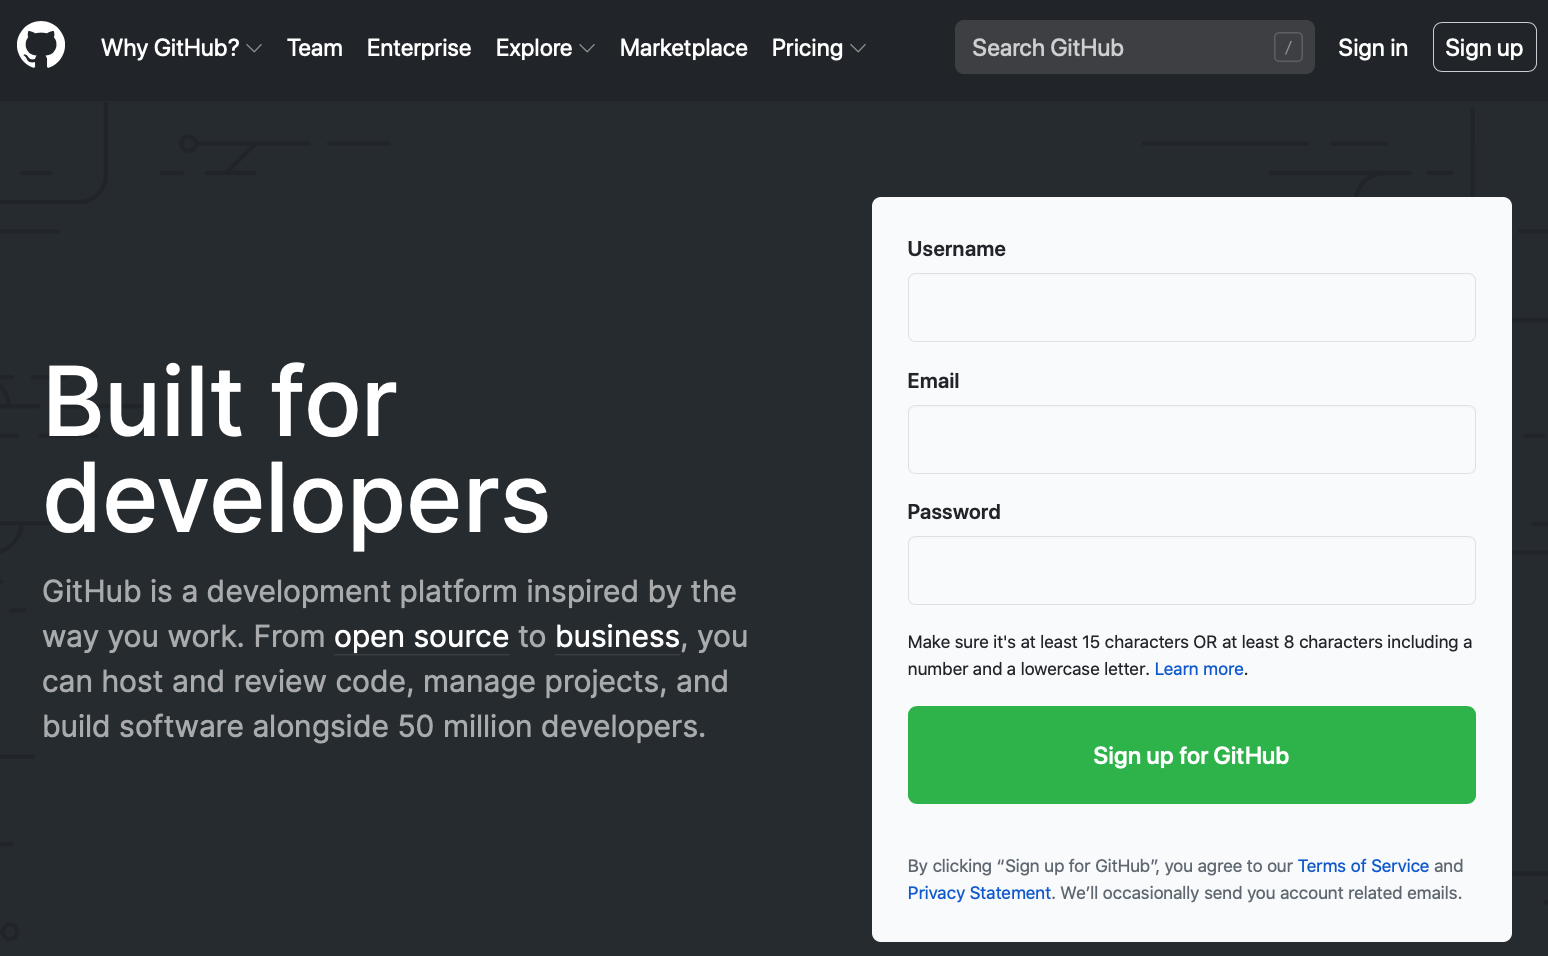
\includegraphics[width=0.75\textwidth]{sec3/github-signup.png}
  \end{figure}

  Pick a username and sign up now with one of your email addresses.

\end{frame}

\begin{frame}<presentation:0>[fragile]
\emptyframetitle

  Once you have an account, go to your profile page. This is in the drop-down menu under the avatar in the top right-hand corner.
  \begin{figure}[h]
    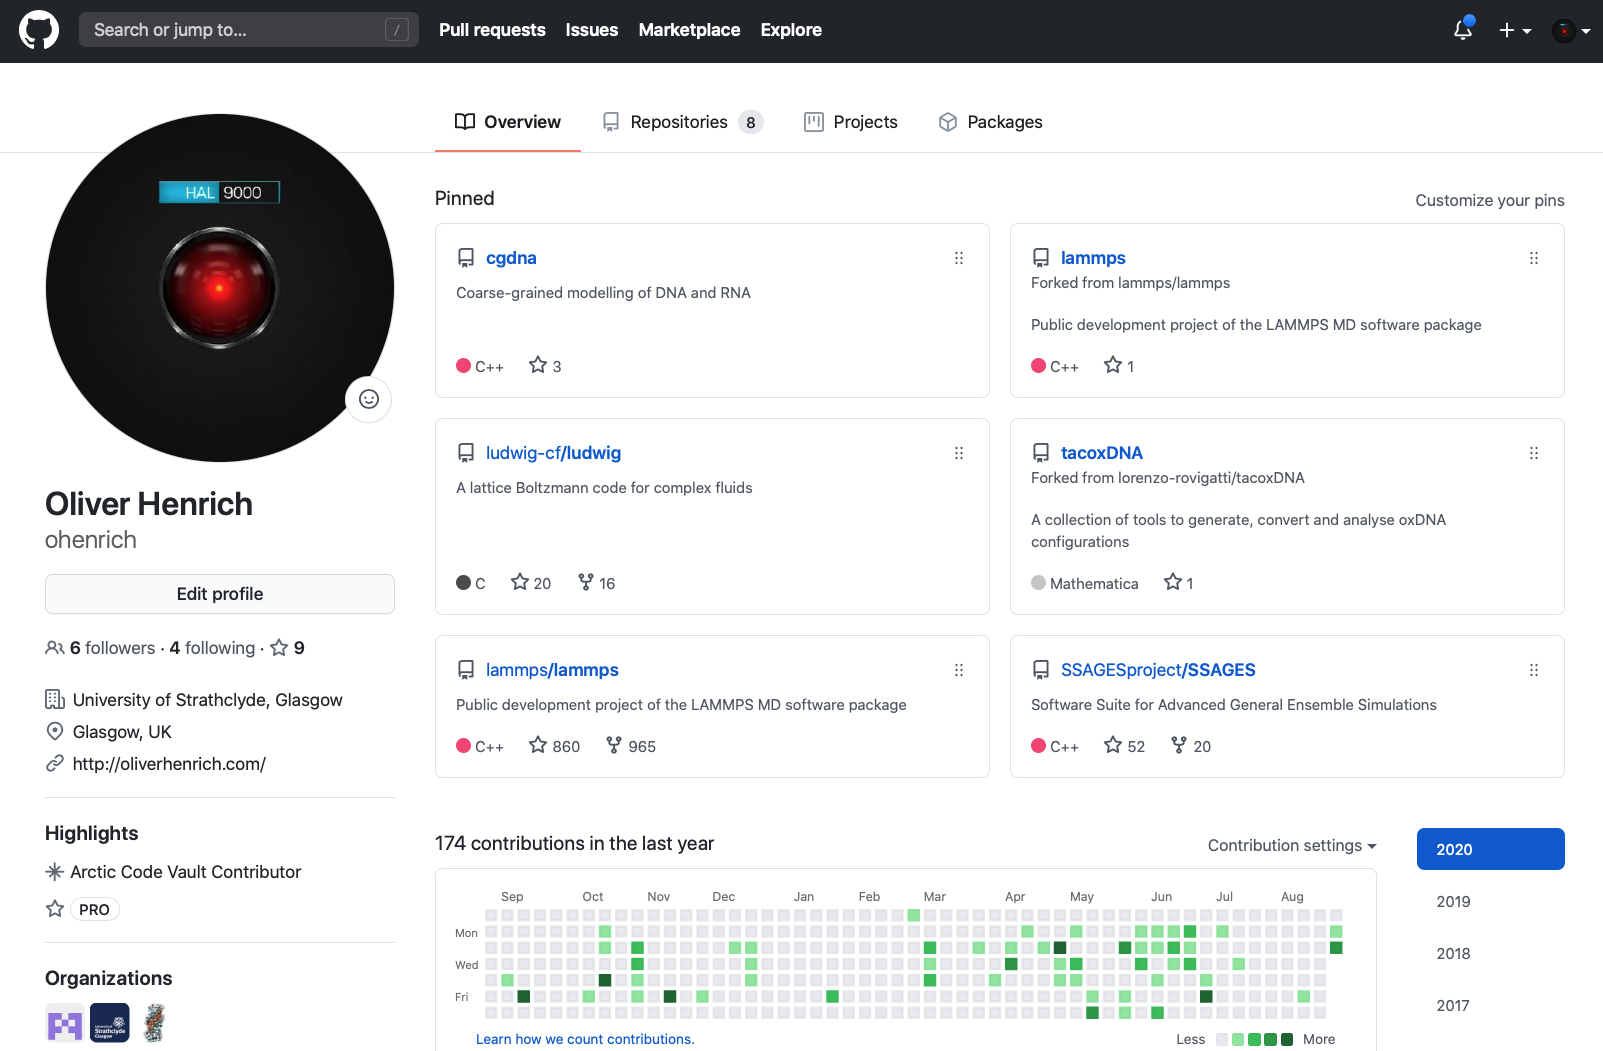
\includegraphics[width=0.75\textwidth]{sec3/github-myprofile.png}
  \end{figure}

\end{frame}

\begin{frame}<presentation:0>[fragile]
\emptyframetitle

  On GitHub, create your first repository.\\[0.25cm]
  Go to \textbf{Repositories}
  \begin{figure}[h]
    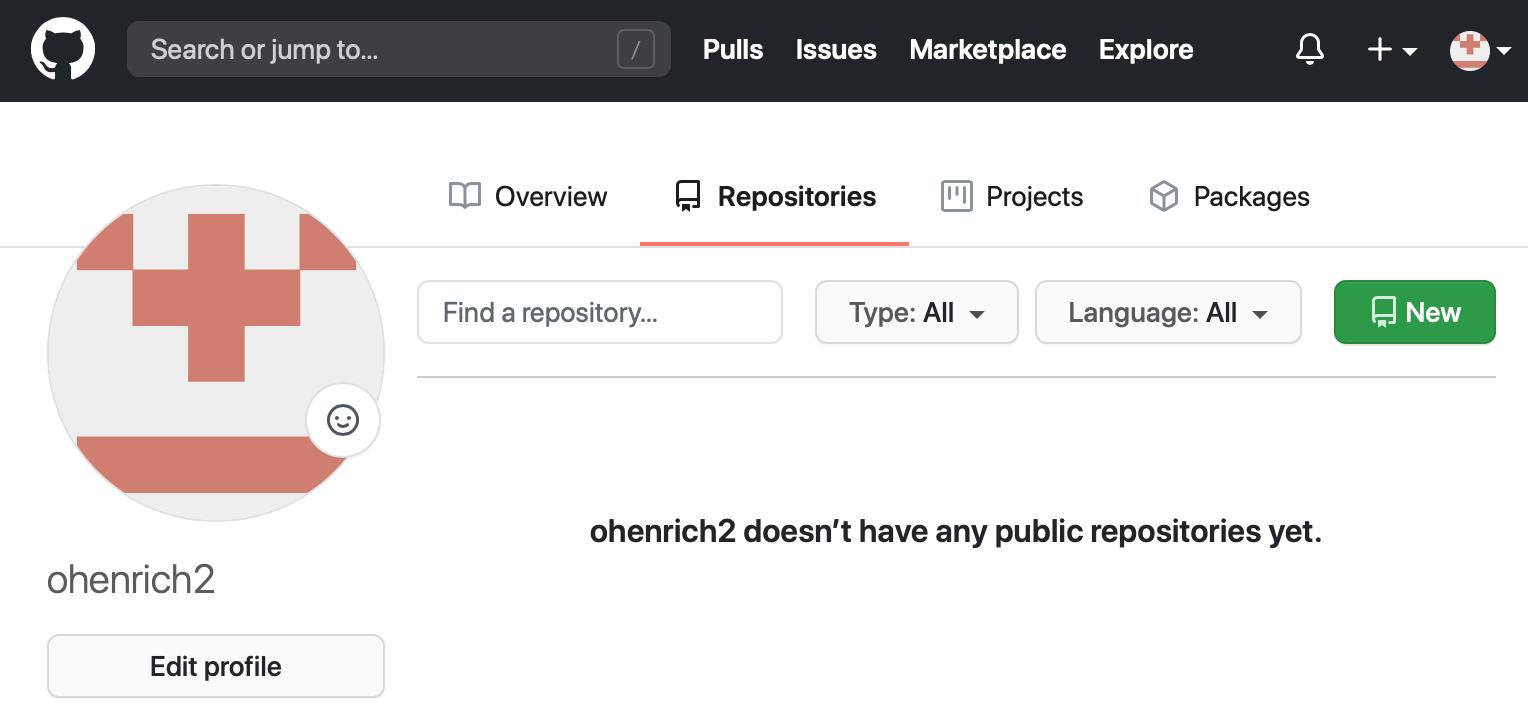
\includegraphics[width=0.75\textwidth]{sec3/github-new-repo.png}
  \end{figure}
  and click on the \textbf{New} button.

\end{frame}


\begin{frame}<presentation:0>[fragile]
\emptyframetitle

  \begin{columns}

    \begin{column}{0.5\textwidth}
      Then chose a name for your repo and create it.
      \begin{figure}[h]
        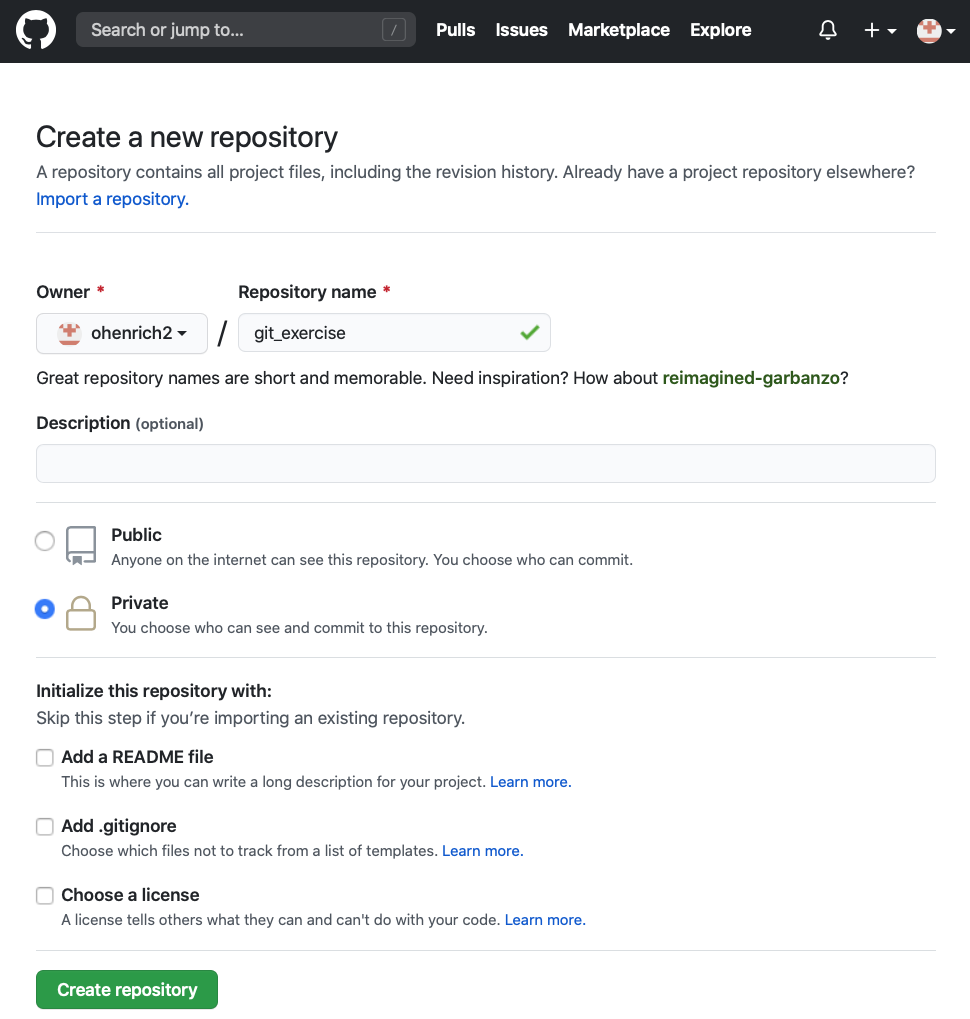
\includegraphics[width=0.95\textwidth]{sec3/github-create-new-repo.png}
      \end{figure}
    \end{column}

    \begin{column}{0.5\textwidth}
      There are a number of options:
      \begin{itemize}
        \item \textbf{Import a repository}: This option is only available if you have another \textit{remote} repo unlike the one you just created
        \item \textbf{Public / Private}: Choose private so only you can interact with it. You can give others access later on.
        \item \textbf{Initialize this repository with}: This adds certain files. Don't do this as we want to import your existing project.
      \end{itemize}
   
\vspace*{0.25cm}   Press the "Create repository" button.
    \end{column}
  \end{columns}

\end{frame}

\begin{frame}<presentation:0>[fragile]
\emptyframetitle

  The next thing you get is a useful overview of what you might want to do next. It contains already the correct code with your individual username, repo URL, etc.

  \begin{columns}
  \begin{column}{0.6\textwidth}
    \begin{figure}[h]
      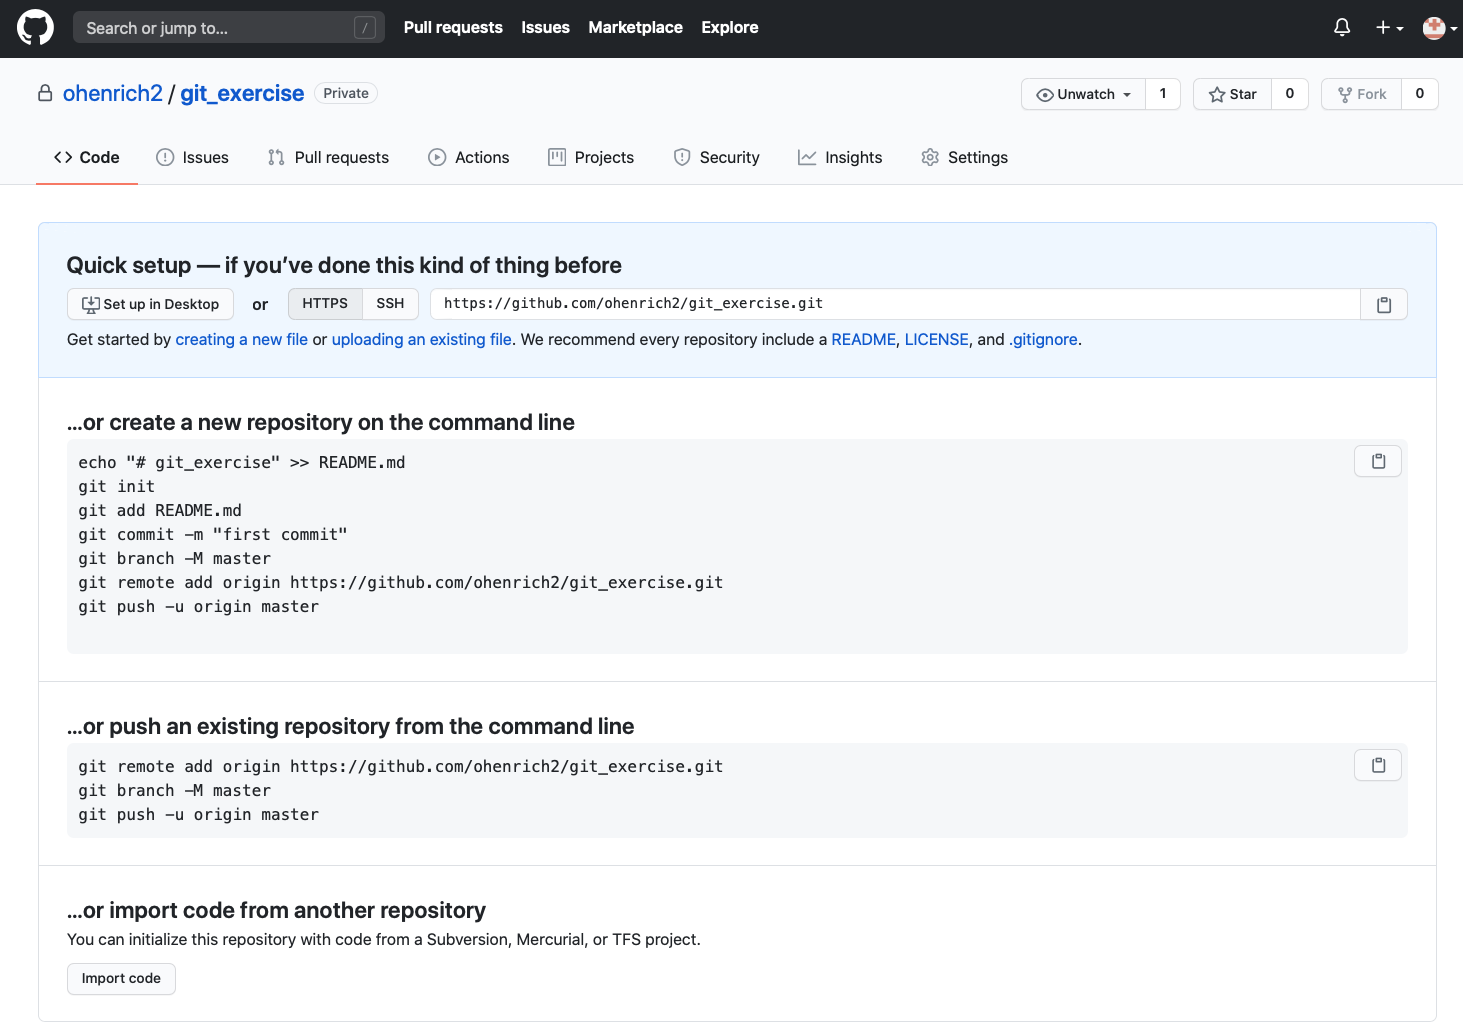
\includegraphics[width=1.0\textwidth]{sec3/github-quick-setup.png}
    \end{figure}
  \end{column}
  \begin{column}{0.4\textwidth}
    \vspace*{3.25cm}
    We are going to do option 2:\\ \textbf{"push an existing repository from the command line"}
  \end{column}
  \end{columns}

\end{frame}


\begin{frame}<presentation:0>[fragile]
\emptyframetitle

  But let's first go back to your profile page and check your "Repositories".\\[0.25cm]

  \begin{figure}[h]
    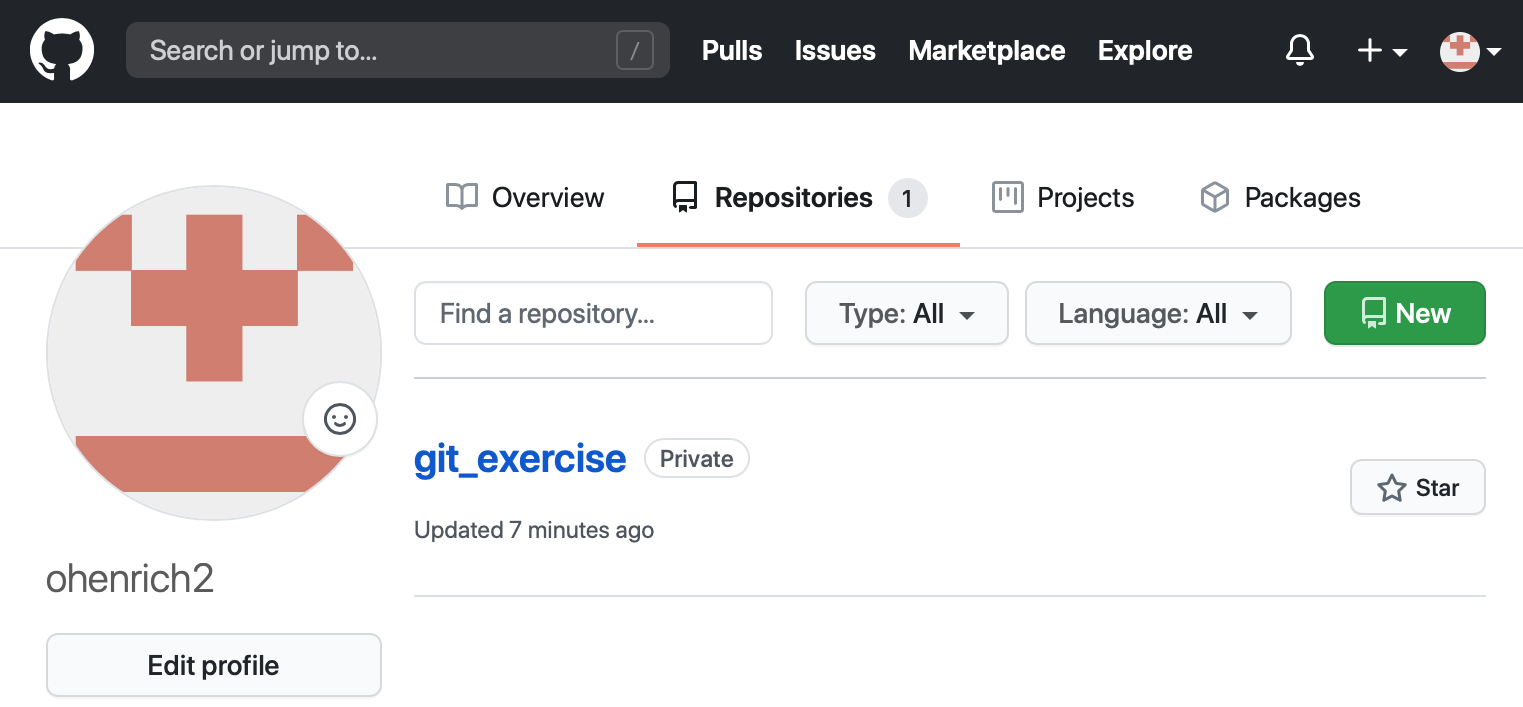
\includegraphics[width=0.75\textwidth]{sec3/github-new-repo-created.png}
  \end{figure}

  When you browse the content of your repo you will see it is completely empty.

\end{frame}


\begin{frame}[fragile]
\emptyframetitle

  Your current situation looks like this

  \begin{figure}[h]
    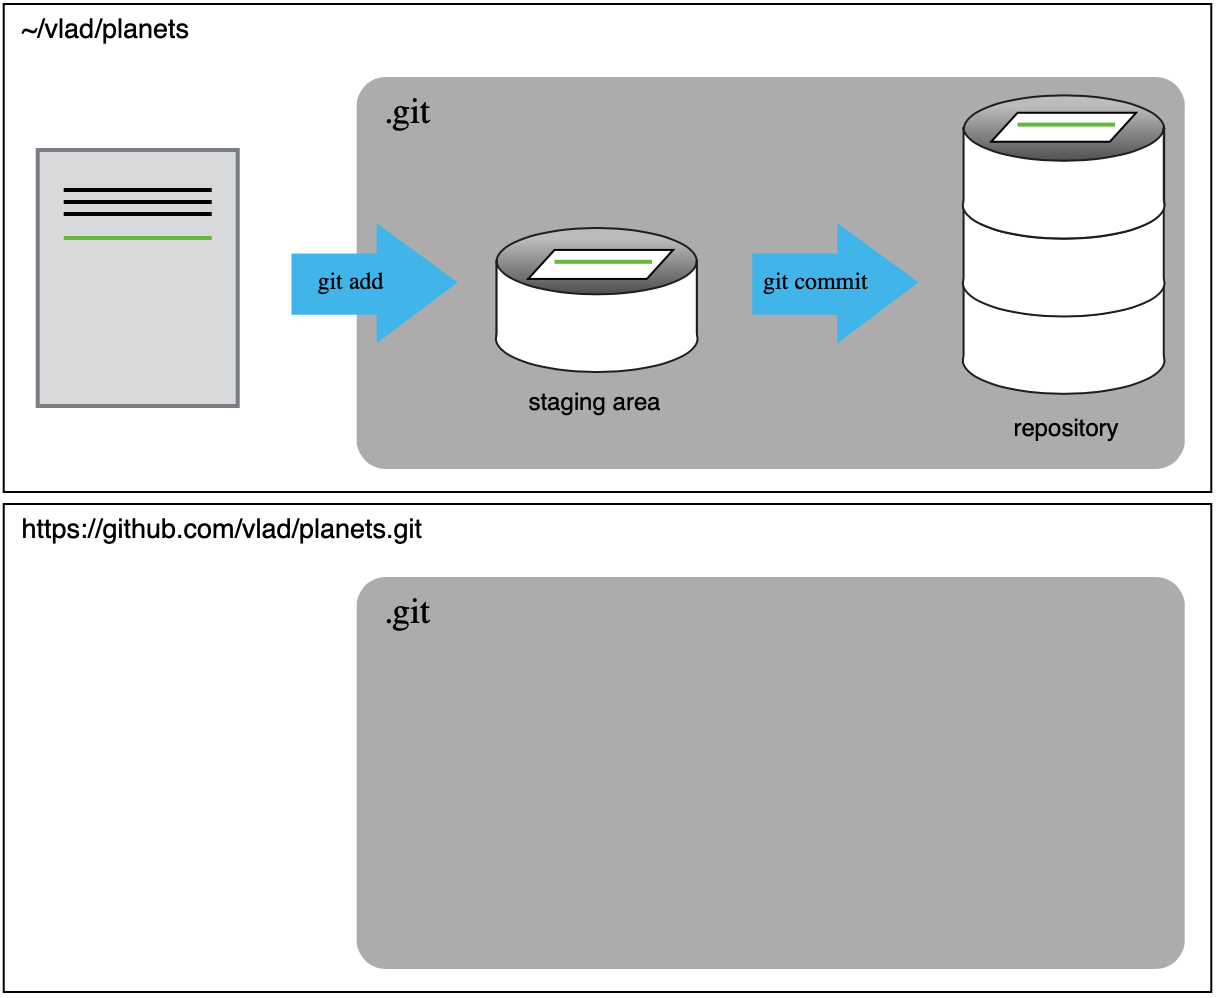
\includegraphics[width=0.55\textwidth]{sec3/git-prior-to-export.png}
  \end{figure}

  We will now \textbf{export your existing local} repo to the \textbf{newly created remote} repo on GitHub.

\end{frame}


\begin{frame}[fragile]
\emptyframetitle


  The full documentation is available on \textbf{\url{https://docs.github.com/en}}, under \textbf{GitHub.com $\rightarrow$ Importing your projects $\rightarrow$ Adding an existing project to GitHub using the command line}.\\[0.25cm]

  \textbf{On GitHub}, look up the URL of your remote repo.\\[0.25cm]

  \textbf{On the command line} change to the directory of your local repo and issue the following sequence of commands replacing username, etc accordingly.
  \begin{lstlisting}[language=bash]
    $ cd git_exercise
    $ git remote add origin https://github.com/username/repo_name.git
    $ git branch -M master
    $ git push -u origin master
  \end{lstlisting}

\end{frame}


\begin{frame}[fragile]
\emptyframetitle

  On GitHub check what's in your remote repository.
  \begin{figure}[h]
    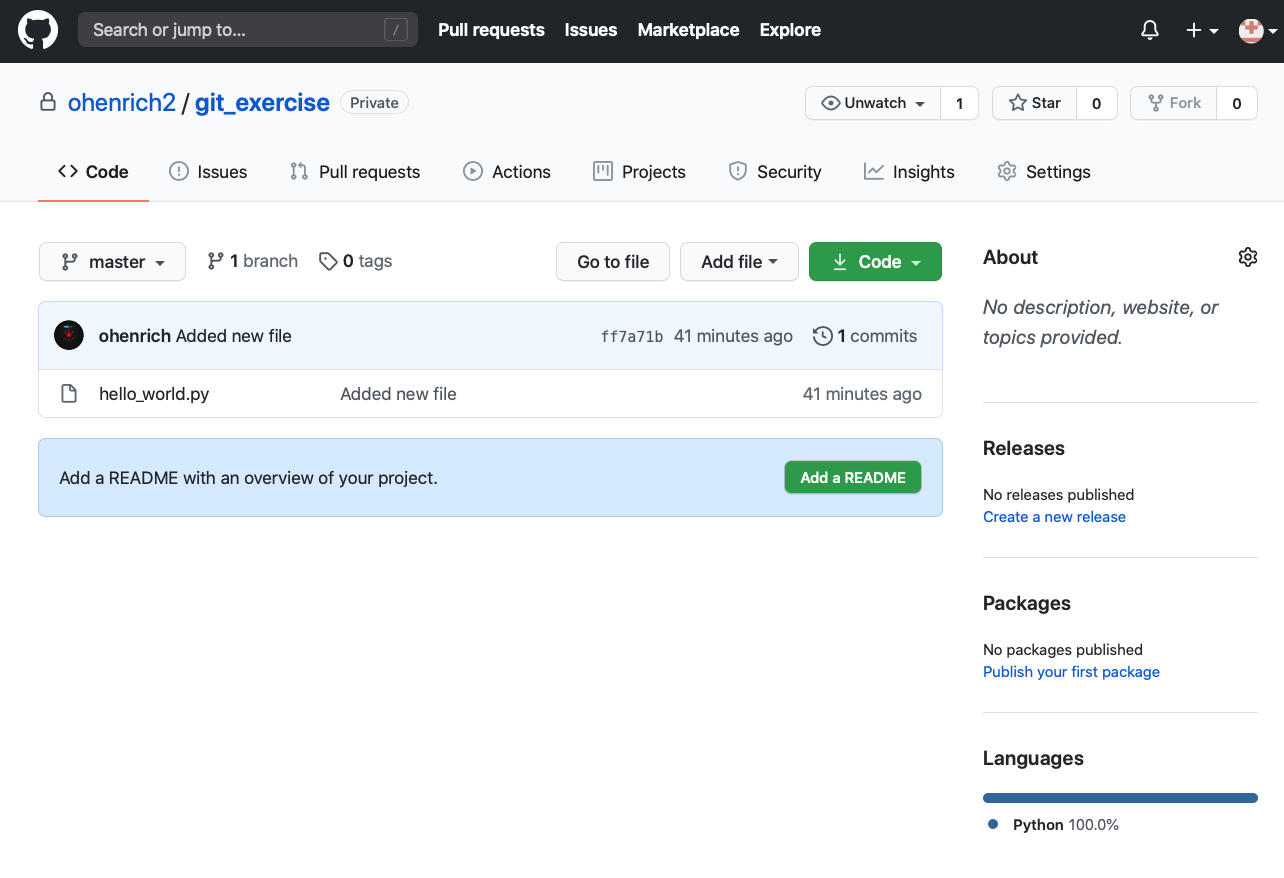
\includegraphics[width=0.85\textwidth]{sec3/github-pushed-existing-repo.png}
  \end{figure}
  \vspace*{-2.5cm}
  \textbf{Hooray!\\[0.25cm] Here is your local code making a\\ first appearance on GitHub!}

\end{frame}


\subsection{Collaborating On GitHub}\hypertarget{sec3.2}{}


\begin{frame}[fragile]
\emptyframetitle

  In \hyperlink{sec3.1}{Section 2.6} we \textbf{exported} an existing \textbf{\textit{local} repository} to your GitHub profile to \textbf{create a remote repository}.\\[0.35cm]

  The inverse process of \textbf{importing} an existing \textbf{\textit{remote} repository} from GitHub is called \textbf{cloning}.\\[0.35cm]

  \textbf{Cloning} produces a \textbf{local copy of the remote repository} on your machine. It requires 
  \begin{itemize}
    \item the \textbf{URL of the remote repository}
    \item the \textbf{\texttt{git clone}} command\\[0.35cm]
  \end{itemize}

  You can modify the local copy and \textbf{push the changes to the remote repository} on GitHub to share them with your collaborators. 
   
\end{frame}


\begin{frame}[fragile]
\emptyframetitle

  First navigate to the repository that you want to clone and click on the "Code" button

  \begin{figure}[h]
    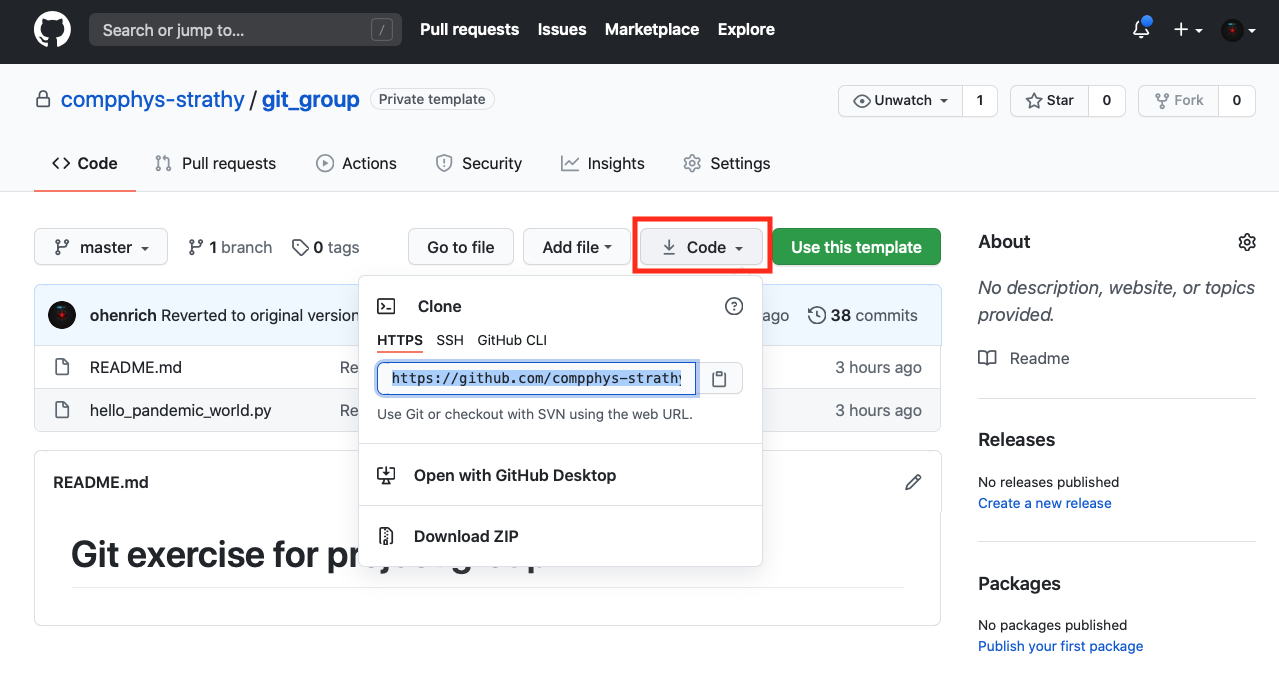
\includegraphics[width=0.75\textwidth]{sec3/github-clone.png}
  \end{figure}

  Copy the URL, e.g. by pressing the button next to it.

\end{frame}


\begin{frame}[fragile]
\emptyframetitle

  On your command line in your working directory issue the following command replacing \textbf{\texttt{URL}} with the actual URL:

  \begin{lstlisting}[language=bash]
    $ git clone URL 
  \end{lstlisting}

  \vspace*{-0.25cm}
  \begin{block}{Output of \texttt{git clone URL}}
  \vspace*{-0.25cm}
    \begin{lstlisting}[language=bash, basicstyle=\footnotesize\ttfamily]
      Cloning into 'git_group'...
      remote: Enumerating objects: 109, done.
      remote: Counting objects: 100% (109/109), done.
      remote: Compressing objects: 100% (79/79), done.
      remote: Total 109 (delta 33), reused 96 (delta 27), pack-reused 0
      Receiving objects: 100% (109/109), 14.32 KiB | 4.77 MiB/s, done.
      Resolving deltas: 100% (33/33), done.
    \end{lstlisting}
  \end{block}

  You can clone the repository it into a different name than the default name (the name on GitHub), e.g. \textbf{\texttt{blablabla}} by adding this after the URL. 

  \begin{lstlisting}[language=bash]
    $ git clone URL blablabla
  \end{lstlisting}
 
\end{frame}

\subsection{Conflicts}\hypertarget{sec3.3}{}

\begin{frame}[fragile]
\emptyframetitle

  \textbf{Conflicts} emerge when \textbf{several} people work on the \textbf{same} code and \textbf{update the remote repo}.\\[0.25cm]

  \begin{figure}[h]
    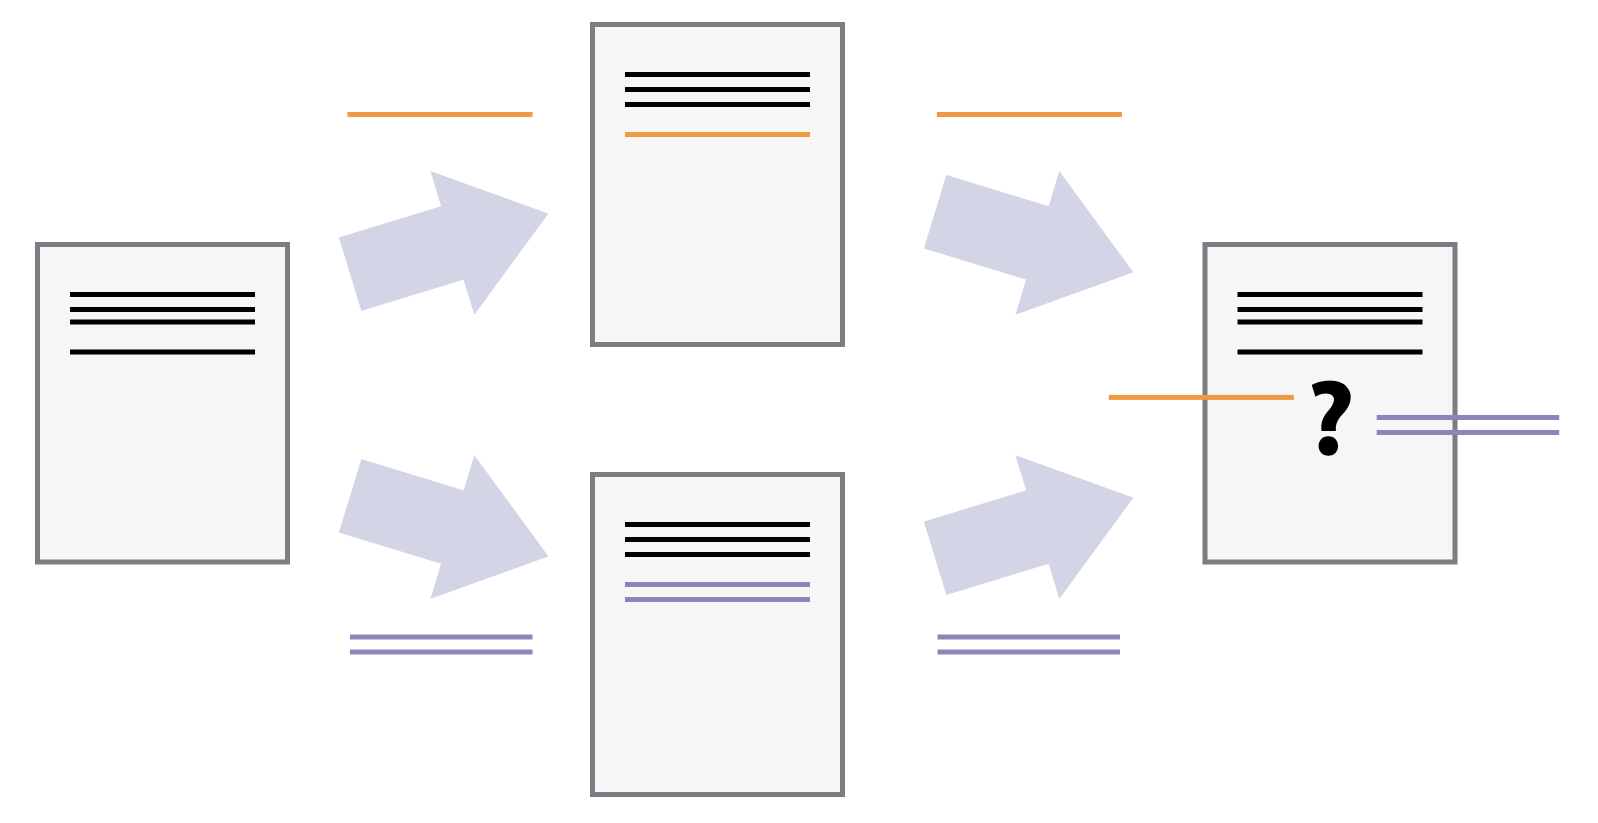
\includegraphics[width=0.7\textwidth]{sec3/git-conflict.png}
  \end{figure}

  The \textcolor{orange}{orange line} and the \textcolor{violet}{purple line} are approximately at the same position in the file. 

\end{frame}

\begin{frame}[fragile]
\emptyframetitle

  Let's look at our \texttt{Hello World!} example.\\[0.cm]

  \begin{columns}
    \begin{column}{0.5\textwidth}

      Your collaborator has checked in the following version:

      \begin{lstlisting}[language=python,basicstyle=\small\ttfamily]
        print('Hello World!')
        print('Hello Scotland!')
        print('Hello City of Glasgow!')
      \end{lstlisting}

    \end{column}

  \begin{column}{0.5\textwidth}

    Your version differs in the last line:
    \vspace{0.25cm}\\
    \begin{lstlisting}[language=python,basicstyle=\small\ttfamily]
      print('Hello World!')
      print('Hello Scotland!')
      print('Hello Greater Glasgow!')
    \end{lstlisting}

    \end{column}
  \end{columns}

  \begin{block}{Output of \texttt{git push origin master}}
    \begin{lstlisting}[language=bash, basicstyle=\tiny\ttfamily]
      To https://github.com/compphys-strathy/git_exercise.git
       ! [rejected]        master -> master (fetch first)
      error: failed to push some refs to 'https://github.com/compphys-strathy/git_exercise.git'
      hint: Updates were rejected because the remote contains work that you do
      hint: not have locally. This is usually caused by another repository pushing
      hint: to the same ref. You may want to first integrate the remote changes
      hint: (e.g., 'git pull ...') before pushing again.
      hint: See the 'Note about fast-forwards' in 'git push --help' for details.
    \end{lstlisting}
  \end{block}


\end{frame}

\begin{frame}[fragile]
\emptyframetitle

  What we have to do is \textbf{pull the changes from the remote repo} on GitHub into your local repo.\\[0.25cm]

  Git \textbf{tries to merge them automatically} into your local copy, and \textbf{if successful this can be pushed} to the remote repo on GitHub.

  \begin{lstlisting}[language=bash]
    $ git pull origin master
  \end{lstlisting}
  \vspace*{-0.25cm}
  \begin{block}{Output of \texttt{git pull origin master}}
    \begin{lstlisting}[language=bash, basicstyle=\tiny\ttfamily]
      remote: Enumerating objects: 5, done.
      remote: Counting objects: 100% (5/5), done.
      remote: Compressing objects: 100% (2/2), done.
      remote: Total 3 (delta 0), reused 0 (delta 0), pack-reused 0
      Unpacking objects: 100% (3/3), 682 bytes | 682.00 KiB/s, done.
      From https://github.com/compphys-strathy/git_exercise
       * branch            master     -> FETCH_HEAD
         dbd3016..5b9c121  master     -> origin/master
      Auto-merging hello_world.py
      CONFLICT (content): Merge conflict in hello_world.py
      <@\textbf{\textcolor{red}{Automatic merge failed; fix conflicts and then commit the result.}}@>
    \end{lstlisting}
  \end{block}

\end{frame}


\begin{frame}[fragile]
\emptyframetitle

  Check what Git has done to your local file.
 \vspace*{0.25cm} 
  \begin{columns}
    \begin{column}{0.59\textwidth}
      \begin{lstlisting}[language=python, basicstyle=\small\ttfamily]
        print('Hello World!')
        print('Hello Scotland!')
        <<<<<<< HEAD
        print('Hello Greater Glasgow!')
        =======
        print('Hello City of Glasgow!')
        >>>>>>> 5b9c121bac
      \end{lstlisting}
    \end{column}
    \begin{column}{0.41\textwidth}
      Our change is preceded by \texttt{\textbf{<<<<<<< HEAD}}.\\[0.2cm]
      Git inserted \texttt{\textbf{=======}} as separator between the conflicting changes.\\[0.2cm]
      The end of the content downloaded from GitHub is marked with \texttt{\textbf{>>>>>>>}}.
    \end{column}
  \end{columns}

  \vspace*{0.5cm}
  We need to \textbf{remove} these markers, \textbf{reconcile} the changes and \textbf{check in a new version}. 

\end{frame}


\begin{frame}[fragile]
\emptyframetitle

  \vspace*{-0.5cm}
  \begin{columns}
    \begin{column}{0.59\textwidth}
      \begin{lstlisting}[language=python, basicstyle=\small\ttfamily]
        print('Hello World!')
        print('Hello Scotland!')
        print('Hello Greater Glasgow!')
        print('Hello City of Glasgow!')
      \end{lstlisting}
    \end{column}
    \begin{column}{0.41\textwidth}
      \vspace*{0.5cm}\\
      We remove the markers and keep both lines.
    \end{column}
  \end{columns}

  Lets' first check the status.
  \vspace*{-0.25cm}

 \begin{columns}
    \begin{column}{0.59\textwidth}
      \begin{block}{Output of \texttt{git status} after editing}
        \begin{lstlisting}[language=bash, basicstyle=\tiny\ttfamily]
      git status
      On branch master
      Your branch and 'origin/master' have diverged,
      and have 2 and 1 different commits each, respectively.
        (use "git pull" to merge the remote branch into yours)

      You have unmerged paths.
        (fix conflicts and run "git commit")
        (use "git merge --abort" to abort the merge)

      Unmerged paths:
        (use "git add <file>..." to mark resolution)
              both modified:   hello_world.py
        \end{lstlisting}
      \end{block}
    \end{column}
    \begin{column}{0.41\textwidth}
      \vspace*{3.5cm}\\
      We are using the last option.
    \end{column}
  \end{columns}

\end{frame}

\begin{frame}[fragile]
\emptyframetitle

  \begin{lstlisting}[language=bash]
    $ git add hello_world.py 
    $ git commit -m 'Resolved conflict'
  \end{lstlisting}

  \vspace*{-0.25cm}
  \begin{block}{Output of \texttt{git commit}}
  \vspace*{-0.25cm}
    \begin{lstlisting}[language=bash]
      [master c7c8fb8] Resolved conflict
    \end{lstlisting}
  \end{block}
 
  \vspace*{-0.25cm}
  \begin{lstlisting}[language=bash]
    $ git push origin master 
  \end{lstlisting}

  \vspace*{0.25cm}

  \textbf{Minimise the number of conflicts by using this workflow}:

  \begin{enumerate}
    \item Update local \hspace*{0.25cm} \texttt{\textbf{git pull origin master}}
    \item Make changes	
    \item Stage changes \hspace*{0.25cm} \texttt{\textbf{git add your\_edited\_file.py}}
    \item Commit changes \hspace*{0.25cm} \texttt{\textbf{git commit -m "Your commit message"}}
    \item Update remote \hspace*{0.25cm} \texttt{\textbf{git push origin master}}
  \end{enumerate}

\end{frame}

% ==============================================================
% --- Git
% ==============================================================
\section{Further Information}\hypertarget{sec3}{}

\begin{frame}[fragile]
\emptyframetitle

  Git is extremely powerful, but also very complex.\\[0.5cm]

  Excellent \textbf{Git tutorial materials} are available on the Software Carpentry website:\\[0.5cm]
  \textbf{\url{http://swcarpentry.github.io/git-novice}}\\[0.5cm]

  \begin{figure}[h]
    
\includegraphics[width=0.95\textwidth]{sec4/software-carpentry.png}
  \end{figure}


\end{frame}



\end{document}
